\chapter{Interstellar Medium}
\section{Cooling}

\begin{figure}[!htbp] 
   \begin{center}$ 
    \begin{array}{cc} 
      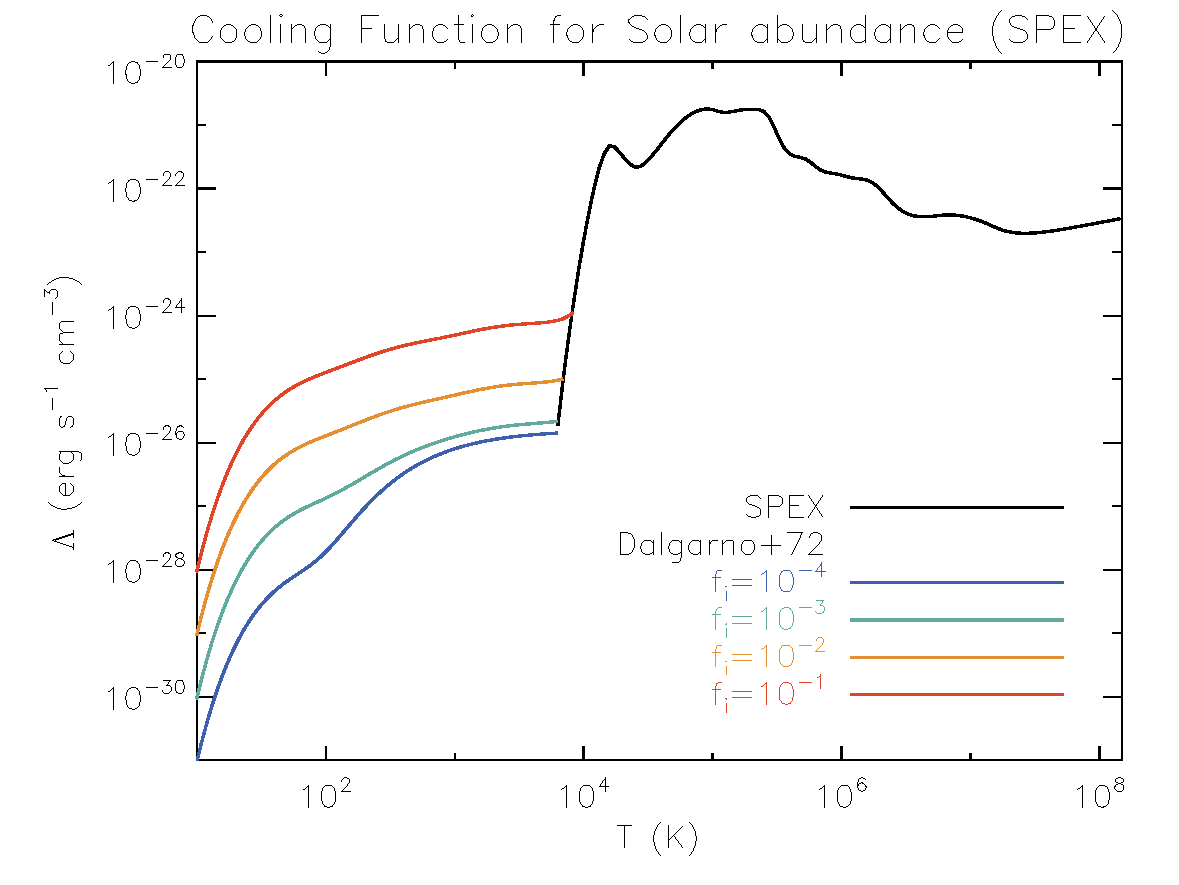
\includegraphics[width=0.5\textwidth]{ISM/spex_cool} &  
      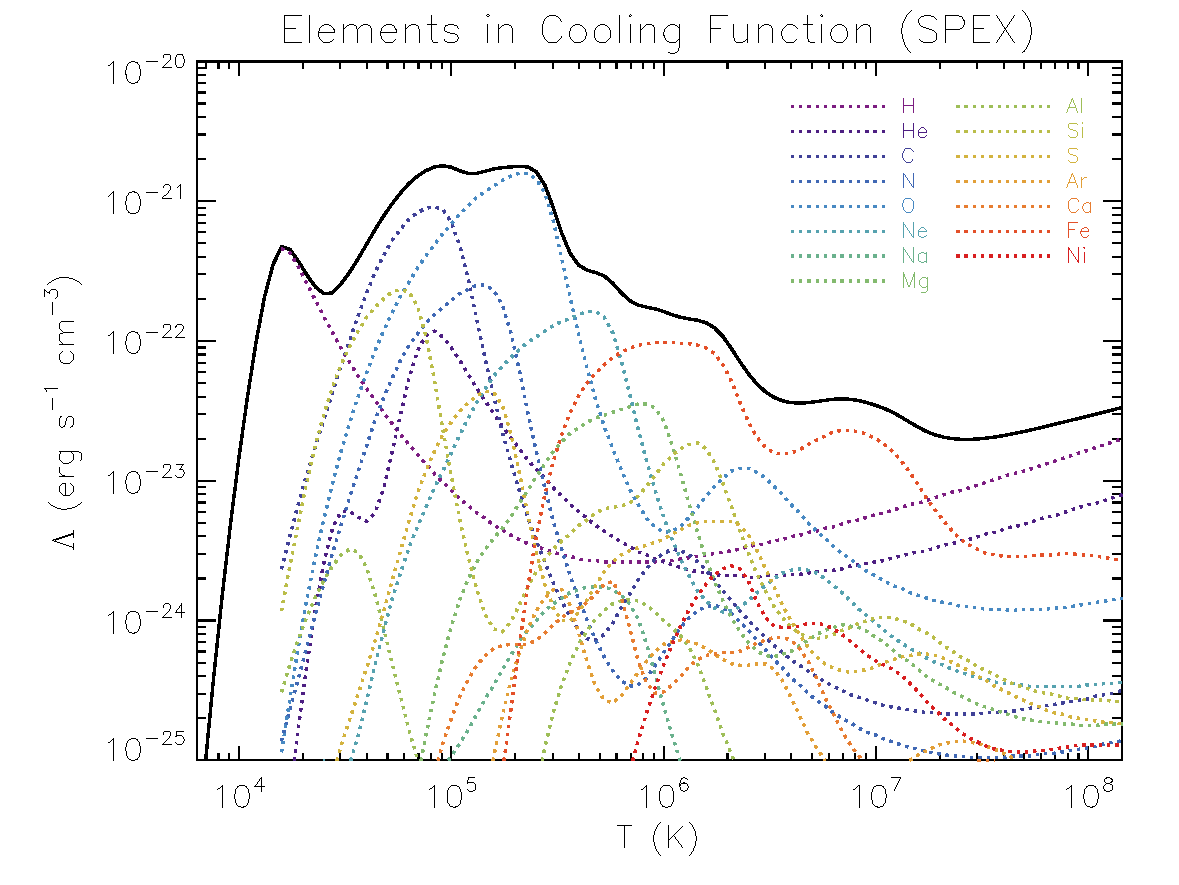
\includegraphics[width=0.5\textwidth]{ISM/spex_cool_elements}    
    \end{array}$ 
   \end{center} 
    \caption{Cooling function in Collisional Ionization Equilibrium (CIE). I made use of SPEX pacakge\cite{Schure:09}. {\it left panel}: The cooling functions in low Temperature ($T < 10^{4}$ K) are computed from \cite{Dalgarno:72}, and the colored lines represent the cooling curves in different ionization fraction ($f_{i}=n_{e}/n_{H}$). {\it right panel}: The contribution of each elements on the cooling curve.} 
   \label{fig:spexCool} 
\end{figure}

\bigskip
\section{Heating}

%\bibliographystyle{apj}
%\bibliography{citations}
